%%%%%%%%%%%%%%%%%%%%%%%%%%%%%%%%%%%%%%%%%
% Journal Article
% LaTeX Template
% Version 1.4 (15/5/16)
%
% This template has been downloaded from:
% http://www.LaTeXTemplates.com
%
% Original author:
% Frits Wenneker (http://www.howtotex.com) with extensive modifications by
% Vel (vel@LaTeXTemplates.com)
%
% License:
% CC BY-NC-SA 3.0 (http://creativecommons.org/licenses/by-nc-sa/3.0/)
%
%%%%%%%%%%%%%%%%%%%%%%%%%%%%%%%%%%%%%%%%%

%----------------------------------------------------------------------------------------
%	PACKAGES AND OTHER DOCUMENT CONFIGURATIONS
%----------------------------------------------------------------------------------------
\documentclass[a4paper,11pt, twoside,twocolumn]{article}
\usepackage{blindtext} % Package to generate dummy text throughout this template 

\usepackage[sc]{mathpazo} % Use the Palatino font
\usepackage[T1]{fontenc} % Use 8-bit encoding that has 256 glyphs
\linespread{1.05} % Line spacing - Palatino needs more space between lines
\usepackage{microtype} % Slightly tweak font spacing for aesthetics
\usepackage{float}
\usepackage[english]{babel} % Language hyphenation and typographical rules
\usepackage{multirow}
\usepackage{multicol}
\usepackage[left=2.5cm,right=2cm,top=2cm,bottom=2cm, hmarginratio=1:1,headheight=14pt,columnsep=15pt]{geometry} % Document margins
\usepackage[hang, small,labelfont=bf,up,textfont=it,up]{caption} % Custom captions under/above floats in tables or figures
\usepackage{booktabs} % Horizontal rules in tables
\usepackage{graphicx}
\usepackage{enumitem} % Customized lists
\usepackage{color}
\usepackage{pdfpages}
\setlist[itemize]{noitemsep} % Make itemize lists more compact
\usepackage{ latexsym }
\usepackage{abstract} % Allows abstract customization
\renewcommand{\abstractnamefont}{\normalfont\bfseries} % Set the "Abstract" text to bold
\renewcommand{\abstracttextfont}{\normalfont\small} % Set the abstract itself to small italic text

\usepackage{fancyhdr} % Headers and footers
\pagestyle{fancy} % All pages have headers and footers
\fancyhead{} % Blank out the default header
\fancyfoot{} % Blank out the default footer
%\fancyhead[C]{Running title $\bullet$ May 2016 $\bullet$ Vol. XXI, No. 1} % Custom header text
\fancyfoot[RO,LE]{\thepage} % Custom footer text

\usepackage{titling} % Customizing the title section
\usepackage{titlesec}
\titleformat{name=\section}{\flushleft\bf\scshape\Large}{\thesection}{.5em}{}
\titleformat{name=\subsection}{\flushleft\bf\scshape\large}{\thesubsection}{.5em}{}
\titleformat{name=\subsubsection}{\flushleft\bf\scshape\normalsize}{\thesubsubsection}{.5em}{}

\usepackage{hyperref} % For hyperlinks in the PDF
\usepackage{amsfonts} % For more logic symbols
\usepackage{amssymb} % For more logic symbols
\usepackage[fleqn]{amsmath} % left aligned math
\usepackage{centernot} % to use not implies
\usepackage{array}
\usepackage{upgreek}
\setlength\parindent{0pt}
%----------------------------------------------------------------------------------------
%	Custom Logic Environment and  Bindings
%----------------------------------------------------------------------------------------
%eq numbering
\makeatletter
\newcommand{\eqnum}[1][]{\leavevmode\hfill\refstepcounter{equation}\label{#1}\textup{\tagform@{\theequation}}}
\makeatother
%environment formating
\newenvironment{logic}
{\begin{minipage}[c]{\linewidth}  \small \vspace{0.5em}\begin{tabbing}}
{\end{tabbing}\end{minipage}\vspace{0.5em}}
%logic shortcuts
\newcommand*\rot{\rotatebox{90}}
\newcommand{\loin}{$\in$}
\newcommand{\lonin}{$\centernot\in$}
\newcommand{\loforall}{$\forall$}
\newcommand{\locontrad}{$\bot$}
\newcommand{\loexists}{$\exists$}
\newcommand{\loand}{$\land$}
\newcommand{\loor} {$\lor$}
\newcommand{\loneq} {$\neq$}
\newcommand{\losimeq} {$\simeq$}
\newcommand{\losubseteq}{$\subseteq$}
\newcommand{\loimplies}{$\implies$}
\newcommand{\lonimplies}{$\centernot\implies$}
\newcommand{\loimpliedby}{$\Longleftarrow$}
\newcommand{\lonimpliedby}{$\centernot\Longleftarrow$}
\newcommand{\losigma}{\text{$\upsigma$}}
\newcommand{\loturns} {$\vDash$}
\newcommand{\lochi}{$\upchi$}
\newcommand{\lophi}{$\upvarphi$}
\newcommand{\lorarrow}{$\rightarrow$}
\newcommand{\lonturns} {$\nvDash$}
\newcommand{\loiff} {$\iff$}
\newcommand{\loleadsto} {$\leadsto$}
\newcommand{\lomapsto} {$\mapsto$}
\newcommand{\locup} {$\cup$}
\newcommand{\lobigcup} {$\bigcup$}
\newcommand{\lotimes} {$\times$}
\newcommand{\loneg}{$\boldsymbol \neg$}
\newcommand{\loexec}[2] {$\lfloor$#1$\rfloor _{\text{#2}}$}
\newcommand{\loconj}[1] {$\bar{\text{#1}}$}
\newcommand{\ablock} {\null\qquad}
\newcommand{\lotiff} {\textit{\textls[-20]{iff}}}
\newcommand{\hr}{\rule{\linewidth}{0.4pt}}
%-----------------------
%----------------------------------------------------------------------------------------
%	TITLE SECTION
%----------------------------------------------------------------------------------------
\setlength{\droptitle}{-4\baselineskip} % Move the title up

\pretitle{\begin{center}\Huge\bfseries} % Article title formatting
\posttitle{\end{center}} % Article title closing formatting
\title{Object Capability Patterns:\\Policies and Specifications} % Article title
\author{%
\textsc{Shu-Peng Loh} \\[1ex] % Your name
\normalsize Imperial College London \\ % Your institution
\normalsize \href{mailto:shu.loh16@imperial.ac.uk}{shu.loh16@imperial.ac.uk} % Your email address
\and % if 2 authors are required, duplicate these 4 lines if more
\textsc{Sophia Drossopoulou}\\[1ex] % Second author's name
\normalsize Imperial College London \\ % Second author's institution
\normalsize \href{mailto:s.drossopoulou@imperial.ac.uk}{s.drossopoulou@imperial.ac.uk} % Second author's email address
}
\date{} % Leave empty to omit a date


\renewcommand{\maketitlehookd}{%
\begin{abstract}
\noindent  We propose a set of higher-order predicate logic to formally specify object-to-object interactions which can then be used to describe reference dynamics in an object-oriented computational model. Using these predicates, we attempt to formally specify the policies of well-established Object-Capability (OCap) patterns within the OCap literature which we have implemented in the capability-safe language Pony. We also offer some preliminary insights on how such specifications can be used in the context of a non-Ocap model by describing the security properties of a pattern built on the Ethereum smart contract programming language Solidity, which we argue implements a form of stack-based access control.\end{abstract}
}
\begin{document}
\raggedbottom
\renewcommand{\ref}[1]{\textit{\autoref{#1}}}
% Print the title
\maketitle

%----------------------------------------------------------------------------------------
%	ARTICLE CONTENTS
%----------------------------------------------------------------------------------------

\section{Introduction}
Recent widespread adoption of distributed ledger technology (blockchain) has created multiple decentralized, distributed computational platforms where millions of dollars are transacted over codified constructs called smart contracts\footnote{For example, as of 10 Aug 2017, Ethereum is a US\$28 billion blockchain platform with an in-built Turing-complete programming language that can be used to create and deploy such contracts.}.
The power of distributed modern computing hence lies in facilitating cooperation between multiple agents, but it comes with risk as an agent is vulnerable to \textit{unexpected} outcomes\footnote{Representing in general any outcome arising from a piece of code execution that has deviated from an agent's original intention or objective independent from code.} from participating in these smart contracts. This might generally arise from two issues: 
\begin{itemize}
\item oversight or misconception of the outcomes of executing a piece of \textit{known} code
\item failure to defend against malicious execution of \textit{unknown} code components\end{itemize}
\noindent These two issue are often closely intertwined in any system of execution that has both trusted and untrusted code components (the second issue is often a result of the first).\\

In recent years the Object-Capability (OCap) model has received increasing attention as a compelling approach to building robust, distributed systems that promote what Miller\cite{miller2006} calls \textit{cooperation without vulnerability}. The OCap model attemps to address these two issues by alleviating security as a separate concern from the mind of the programmer, by leveraging the object-oriented programming paradigm and imposing certain prohibitions.
%----------------------------------------------------------------------------------------
%   OCap Model
%----------------------------------------------------------------------------------------
\section{OCap Model}
\subsection{From Object to Capability}
The OCap model uses the reference graph of the objects as the access graph, and strictly requires objects to interact with each other only by sending messages on object references\cite{miller2003b}. When these references cannot be forged in the system, and when there there are no default globally accessible objects (for an object to be globally accessible, the reference to use that object has to be \textit{explicitly} granted to every object globally), then it becomes necessary that one needs to obtain references to objects in order to call the associated methods of the object.  Object references therefore embody authority, and we use the word capability to describe the encapsulation of both reference (designation) and authority which are unforgeable. 

\subsection{From Capability to Object-Capability}
Origins of capabilities date back to Dennis and Van Horn\cite{dennis1966}'supervisor as a mechanism of protecting low-level resources like memory segments. Early attempts to implement the capability model include the MIT PDP-1 computer and the CAL-TSS system. The capability model was then extended by the early operating system designers of HYDRA\cite{wulf1974} into a protected ability to invoke arbitrary services provided by other processes. Capabilities were later implemented on computer and operating systems such as CAP\cite{wilkes1979}, KeyKOS\cite{hardy1985}, and EROS\cite{shapiro1999}. More recent work includes the Capsicum kernel framework that provides capabilities support for UNIX\cite{watson2010}, and Google's open-source capabilities-based operating system Fuchsia OS\cite{matte2017}. The development of capabilities and a thorough examination of the object-capability model with the capability-safe programming language E, can be found in Miller's PhD thesis\cite{miller2006}.

\subsection{OCap Languages}
\begin{itemize}
\item Joe-E (inspired by Java)
\item Emily (inspired by OCaml)
\item Caja (inspired by JavaScript)
\item E
\item Pony
\end{itemize}
\subsubsection{Language Restrictions}
\subsection{OCap Patterns}
An OCap pattern is a concrete representation of the OCap model and comprises a set of objects connected to each other by capabilities. Objects interact with each other by sending messages on capabilities. An OCap pattern may be visualised as a directed graph---nodes represent objects, and each edge from an object o to another o' represents o holding a capability that allows it to directly access o'.
%----------------------------------------------------------------------------------------
%   Formal Specifications
%----------------------------------------------------------------------------------------
\newpage
\section{Formal specifications}
\subsection{Definitions}\noindent
We borrow liberally the definitions of runtime state, module and arising configurations from the appendix of \cite{drossopoulou2015b}.\\
\textbf{Runtime state:}
 \losigma\ consists of a stack frame \lophi, and a heap \lochi. A stack frame is a mapping from receiver (this) to its address, and from the local variables (VarId) and parameters (ParId) to their values. Values are integers, the booleans true or false, addresses, or null. The heap maps addresses to objects. Objects are tuples consisting of the class of the object, and a mapping from field identifiers onto values.\\
 
 \begin{logic}[Runtime state]
\losigma\ \loin\ state = frame \lotimes\ heap \\
\lophi \loin\ frame = StackId $\rightarrow$ val \\
\lochi \loin\ heap = addr $\rightarrow$ object \\
v \loin\ val = \{\texttt{null}, \texttt{true}, \texttt{false}\} \locup\ \textit{addr} \locup\ $\mathbb{N}$ \\
StackId = \{\textit{this}\} \locup\ VarId \locup\ ParId \\
object = ClassId \lotimes (FieldId $\rightarrow$ val)\\
\end{logic}

\textbf{Module:}

\begin{logic}
M \loin\ Module = ClassId \locup\ SpecId\\\ablock\qquad\qquad\quad $\rightarrow$ \\
\ablock \qquad \qquad \quad (ClassDescr \locup\ Specification)
\end{logic}

\textbf{Execution:}\\
\begin{logic}\end{logic}



\textbf{Arising State Configurations}\\
\begin{logic}\end{logic}


\subsubsection{MayAccess Definitions}
We define in total four flavours of \textit{MayAccess} predicates that are inspired by the work in Drossopoulou et al.\cite{drossopoulou2015b}, but our four MayAccess predicates extend and modify the definition in \cite{drossopoulou2015b} to more precisely capture the different configurations of access in terms of mode and time: 
\begin{itemize}
\item Mode: directly ($Dir$) or indirectly ($Ind$)
\item Time: now ($Now$) or eventually ($Eve$)
\end{itemize}
and are broad enough to describe both non-OCap and OCap models:

\begin{logic}
\hr\\
\textsc{\normalsize *Four MayAccess Definitions}\\\vspace{0.5em}
M,\losigma\ \loturns\ \=MayAccess$^{Dir,Now}$(x,e) \loiff \\
\>\loexists f. \loexec{x.f}{\losigma} = \loexec{e}{\losigma}
\loor \\
\> (\losigma(this) = \loexec{x}{\losigma} \loand\ \loexists y. \losigma(y) = \loexec{e}{\losigma})\\
\\
 M,\losigma\ \loturns\ \=MayAccess$^{Dir,Eve}$(x,e) \loiff \\
\>\loexists \losigma' \loin Arising(M,\losigma).\\
\>M,\losigma'\ \loturns\ MayAccess$^{Dir,Now}$(x,e)\\
\\
M,\losigma\ \loturns\ \=MayAccess$^{Ind,Now}$(x,e) \loiff \\
\>\loexists \loconj{f}. \loexec{x.\loconj{f}}{\losigma} = \loexec{e}{\losigma}
\loor \\
\>(\losigma(this) = \loexec{x}{\losigma} \loand\ \loexists y. \losigma(y.\loconj{f}) = \loexec{e}{\losigma})\\
\\
M,\losigma\ \loturns\ \=MayAccess$^{Ind,Eve}$(x,e) \loiff \\
\>\loexists \losigma' \loin Arising(M,\losigma).\\
\>M,\losigma'\ \loturns\ MayAccess$^{Ind,Now}$(x,e)\\
\hr
\end{logic}

where, we say MayAccess$^{Dir,Now}$(x,e) holds \lotiff\ in some current state \losigma, we have a field in x that points to e, or that we have x as a receiver in \losigma\ and there exists some y in the same \losigma\ that points to e. We also say MayAccess$^{Ind,Now}$(x,e) holds \lotiff\ in some current state \losigma, we have a \textit{series of fields} in x that leads to e, or that we have x as a receiver in \losigma\ and there exists some y with a series of fields in the same \losigma\ that leads to e. Lastly, the 'eventual' definitions of the two predicates are then defined as there existing an arising configuration \losigma' from \losigma, where the 'now' definitions hold at \losigma'.\\

Note that MayAccess$^{*,Now}$ holds imply MayAccess$^{*,Eve}$ holds, since an eventual state \losigma' that arises from \losigma\, can refer to \losigma, and therefore, the 'now' definitions implies and are stronger than the 'eventual' definitions. Also since a series of fields \loconj{f}\ can mean a singular field f, MayAccess$^{Dir,*}$ holds imply MayAccess$^{Ind,*}$ holds, and therefore the 'direct' definitions are stronger than the 'indirect' definitions. We surmarise the relationships between the four flavours of MayAccess in \ref{MayAccessRelations}.\\
\begin{table}[htb]
\small
\caption{MayAccess Relations}
\centering
\begin{tabular*}{\linewidth}{c|ccc}\toprule
& \bf Now & & \bf Eventually\\
\hline
\multirow{5}{*}{\rot{\bf Indirect \enspace Direct \:}} & \multirow{2}{*}{MayAccess$^{Dir,Now}$} & \loimplies & \multirow{2}{*}{MayAccess$^{Dir, Eve}$} \\
& & \lonimpliedby &  \\
& \rot{\loimpliedby} \rot{\lonimplies}& &\rot{\loimpliedby} \rot{\lonimplies} \\
& \multirow{2}{*}{MayAccess$^{Ind,Now}$} & \loimplies & \multirow{2}{*}{MayAccess$^{Ind, Eve}$} \\
& & \lonimpliedby &\\
\label{MayAccessRelations}
\end{tabular*}
\end{table}

Note that without imposing any further assumptions (such as those from the OCap model), we have defined \textit{both} MayAccess$^{Dir,Now}$(x,e) and MayAccess$^{Ind,Now}$(x,e) to mean forms of very weak access---that a directed path exists from x to e, and that we do \textit{not} imply that such a path is \textit{traverseable} by x. By a path being traverseable from x to e, we mean that x has a method that upon invocation, can lead to a method invocaton in e, and therefore x can interact with e, and possibly, modify e. These MayAccess definitions by themselves represent mere paths, or mere \textit{possibilities} of object interaction---they do \textit{not} imply that interaction would succeed. We therefore need another predicate describes method invocation between objects. 

\subsubsection{MayAffect Definitions}
With our access predicates in place, we define a \textit{MayAffect} predicate that describe what it means for x to be able to affect e:\\
\begin{logic}
\hr\\
\textsc{\normalsize *MayAffect Definition}\\\vspace{0.5em}
M,\losigma\ \loturns\ \=MayAffect(x,e) \loiff \\
\> \losigma(this) = \loexec{x}{\losigma} \loand\ \loexists \losigma'\loin Arising(M,\losigma)\\
\> \loand\ \losigma'(this) = \loexec{e}{\losigma'}\\
\hr
\end{logic}

where we say MayAffect(x,e) holds \lotiff\ we have x as a receiver in some state \losigma, and in some arising state \losigma' from \losigma, we have e as a receiver in \losigma'. This means that there must exist some method in x that upon invocation, will result in some state \losigma' where e is the receiver in the state \losigma'. Other possible definitions for MayAffect and why we have settled for the definition above arguing about method invocation, can be found in the Appendix (\ref{appendix}).\\


\subsection{Object-Oriented Paradigm}
 
As our paper focuses on security between trusted and untrusted objects, we shift our use of these predicates to an object-oriented paradigm. So, what do our above definitions mean in an object-oriented world?

\begin{logic}
\hr\\
\textsc{\normalsize *Object as Receiver Nec. Cond.}\\\vspace{0.5em}
M,\losigma\ \loturns\ \=\losigma(this) = \loexec{o$_x$}{\losigma}\loimplies \\
\> \loexists \losigma*,m,\loconj{a}. M,\losigma*, o$_x$.m(\loconj{a}) \loleadsto\ \losigma\\
\hr
\end{logic}

We first make clear that for an object to be a receiver in a particular state \losigma, we require a method to exist in the object in a prior state \losigma* that upon invocation can lead to state \losigma. This follows from our definition of execution.
Let us illustrate this with an example where there is a particular state \losigma\ of the system with a configuration of 3 objects o$_1$, o$_2$, and o$_3$. In this example, to illustrate object encapsulation, we assume all fields in objects are private. o$_1$.next is a private field that holds the object reference of o$_2$, and o$_2$.next is a private field that holds the object reference of o$_3$. In this example:
\begin{itemize}
\item M,\losigma ~\loturns MayAccess$^{Ind,Now}$(o$_1$,o$_3$) holds true, regardless of whether we know o$_1$ can invoke any methods on o$_3$.

\item If o$_1$ contains no method that can invoke o$_2$, or o$_2$ has no methods that can be invoked externally, then according to our definitions, we say M,\losigma ~\loturns \loneg MayAffect(o$_1$,o$_2$), meaning that o$_1$ cannot affect o$_2$.

\item If o$_1$ contains a method that can invoke o$_2$, and o$_2$ contains some public method that can be invoked externally which is empty and does nothing, but o$_2$ contains no method that can invoke o$_3$, then according to our definitions, we mean M,\losigma ~\loturns\ \loneg MayAffect(o$_2$,o$_3$), since we know o$_2$ does not have any way of invoking o$_3$. We also mean M,\losigma ~\loturns\ MayAffect(o$_1$,o$_2$) to hold, because given this configuration, we know o$_1$ has a method that can invoke o$_2$ and, that o$_2$ has a public method that can be invoked, even if it does nothing.
\end{itemize}
Note that if we assume all fields are private, for an object o to \textit{eventually modify} an object o', it requires:
\begin{itemize}
\item there exist a method in o that can eventually invoke a method in o'
\item there eventually exist a method in o' that can be invoked externally to modify its own internal state
\end{itemize}
Our MayAffect(o,o') predicate however, is not concerned whether or not the state o' is modified ---the fact that a method in o' can be eventually invoked by o is good enough grounds for us to mean that o can affect o'. Our justification is that in the object-oriented paradigm, programmers almost always enforce security of a sensitive field in a protected object to be declared private, and define some public method in the object that can modify the concerned private field based on some condition:
\begin{logic}
\hr\\
\textsc{\normalsize *Private Field Definition}\\\vspace{0.5em}
M,\losigma\ \loturns\ \=PrivField(o,f) \loiff\\
\>$[$\loexists \losigma'\loin Arising(M,\losigma) \loand\ \loexec{f}{\losigma'}\loneq\loexec{f}{\losigma} \loimplies \\
\> \loexists m,\loconj{a}. M,\losigma, o.m(\loconj{a}) \loleadsto\ \losigma'$]$\\
\hr
\end{logic}
Hence, the question of whether an untrusted object can modify a private field in a protected object can often be expressed as a question of whether the untrusted object can invoke a method in the protected object. Furthermore, given our definitions of PrivField and MayAffect, we can derive a lemma that states that a necessary condition for modification of a private field in o$_x$ is the existence of some arbitrary object o* that can affect o$_x$, where it is also possible that o* can refer to o$_x$. Proving the falsity of our MayAffect predicate is therefore sufficient to prove that all private fields in o$_x$ cannot be modified:
\begin{logic}
\hr\\
\textsc{\normalsize *Private Field Modification Lemma}\\\vspace{0.5em}
M,\losigma\ \loturns\ \loforall \losigma',f. \=$[$\losigma'\loin Arising(M,\losigma) \loand\ \loexec{f}{\losigma'}\loneq\loexec{f}{\losigma}\\
\>\loand\ PrivField(o,f) \loimplies \\
\>\loexists o*. M,\losigma\ \loturns\ MayAffect(o*,o)\\
\hr
\end{logic}

Therefore, our MayAffect(o,o') requires:
\begin{itemize}
\item there exist a method in o$_x$ (\losigma(this)=\loexec{o}{\losigma}) that can eventually invoke a method in o' (\loexists \losigma'\loin Arising(M,\losigma) \loand\ \losigma'(this) = \loexec{o'}{\losigma'})
\item which by collorary means there eventually exist a method in o' that can be invoked externally \losigma'(this) = \loexec{o'}{\losigma'}
\end{itemize}

Note, that in some languages like JavaScript, methods can be added to objects dynamically at run-time, such that a method of an object that does not exist in some current state can potentially exist in some eventual later state. However, if we are operating in a language that does not allow dynamically adding of methods to objects, or that the protected object o$_y$ is defined such that methods cannot be added dynamically to it, proving there does not exist a public method now in o$_y$ is sufficient to prove that there will not eventually exist a public method in o$_y$:

\begin{logic}
\hr\\
\textsc{\normalsize *No dynamic adding of methods to objects.}\\\vspace{0.5em}
M,\losigma\ \loturns\
\= \loforall o,\losigma',m,\loconj{a$_\losigma$},\loconj{a$_{\losigma'}$}.\\
\>[ \losigma'\loin Arising(M,\losigma) \loand\ \losigma'(o.m(\loconj{a$_{\losigma'}$}))\\
\>\loimplies \losigma(o.m(\loconj{a$_\losigma$})) ]\\
\hr 
\end{logic}
\subsubsection{Domination}
Here, we introduce the concept of domination that is inspired by the work on ownership types by Clarke et al.\cite{clarke1998}, where they define that the owner o of an object o' dominates o' in the object graph such that for any path p from some arbitrary object o'' to o', either o'' belongs to the set of owners or that p passes through o. Similarly, we say that a set S dominates x \lotiff\ for every object X* in the system that has a path to x, X* must either have a path to some arbitrary object y that is a member of the set S, or X* belongs to the set S.
\begin{logic}
\hr\\
\textsc{\normalsize *Domination Definition (DOM)}\\\vspace{0.5em}
M,\losigma\ \loturns\ \=Dom(S,x) \loiff \\
\> \loforall X*. $[$\=MayAccess$^{Ind,Now}$(X*,x) \loimplies\\
\> \>\loexists y\loin S. \=MayAccess$^{Ind,Now}$(X*,y) \loor\ X*\loin S$]$\\
\hr
\end{logic}


\subsubsection{Corollaries}

\begin{logic}
\hr\\
\textsc{\normalsize *Path-Execution Condition (PEC)}\\\vspace{0.5em}
M,\losigma\ \loturns\
\= MayAffect(o,o') \loimplies \\
\> MayAccess$^{Ind,Eve}$(o,o')\\
\hr
\end{logic}

\begin{logic}
\hr\\
\textsc{\normalsize *Global Path Chain (GPC)}\\
M,\losigma\ \loturns\ \=MayAccess$^{Ind,Now}$(o,o')\\
\>\loiff\\
\>\loexists X*. $[$\=MayAccess$^{Ind,Now}$(o,X*) \loand\\
\>\> MayAccess$^{Dir,Now}$(X*,o')$]$\\
\hr
\end{logic}

\begin{logic}
\hr\\
\textsc{\normalsize *Global Path Chain II (GPC II)}\\
M,\losigma\ \loturns\ \=MayAccess$^{Ind,Now}$(o,o') \loand\ Dom(S,o')\\
\>\loimplies\\
\>\loexists X*\loin{S}. $[$\=MayAccess$^{Ind,Now}$(o,X*) \loand\\
\>\> MayAccess$^{Dir,Now}$(X*,o')$]$\\
\hr
\end{logic}

\begin{logic}
\hr\\
\textsc{\normalsize *Global Execution Chain (GEC)}\\
M,\losigma\ \loturns\ \=MayAffect(o,o')\\
\> \loiff\\
\> \loexists X*. $[$\=MayAffect(o,X*) \loand\\
\>\>MayAffect(X*,o')$]$\\
\hr
\end{logic}

\begin{logic}
\hr\\
\textsc{\normalsize *Global Execution Chain II (GEC II)}\\
M,\losigma\ \loturns\ \=MayAffect(o,o') \loand\ Dom(S,o')\\
\> \loimplies\\
\> MayAccess$^{Ind,Eve}$(o,o') \loand\\
\> \loexists x\loin{S}. $[$\=MayAffect(o,x) \loand\\
\> \>MayAffect(x,o')$]$\\
\hr
\end{logic}
\subsubsection{Lemmas}
\begin{logic}
\hr\\
\textsc{\normalsize *Object Existence Lemma (OEL)}\\
\textit{if z exists in \losigma,} \\
\loturns\ M,\losigma\ \loturns\ \=MayAccess$^{Ind,Now}$(z,z) is true \loand\\
\loturns\ M,\losigma\ \loturns\ \=MayAccess$^{Dir,Now}$(z,z) is true \loand\\
\loturns\ M,\losigma\ \loturns\ \=MayAffect(z,z) is true\\
\hr
\end{logic}

\subsection{OCap Specifications}


\subsubsection{What is protection?}
In an object-oriented world, security concerns between objects are often a question of whether what one object can do to another object in \textit{any} eventual state of a system. Because an object encapsulates both state and behaviour, strictly speaking, security of an object should govern over both the integrity of the object's fields (object state) and whether the objects' methods can be called (object behaviour). Our \textit{MayAffect} predicate enables a discussion of protection of behaviour\footnote{ Our MayAffect is too strong to reason specifically which behaviours can be called. This is however not a big issue in \textit{pure} OCap systems, where often giving away the capability of an object typically means allowing \textit{all} public behaviours of the object to be called without distinction.}
and because we assume that protected objects should have fields that are privately encapsulated, we only need to focus our reasoning on object to object method invokations as a security concern. With these simplifications, protection for us then becomes solely a matter of whether we can allow or deny an object to invoke a method of another object. To help us reason about protection, we first formalize our assumptions and the rules of OCap using our predicates in \ref{ocaprules} which will help guide us in constructing our necessary conditions for MayAffect later in \ref{protection}.

\subsection{Formal specifications in the OCap Model}\label{ocaprules}

\subsubsection{Passing object references}
Objects cannot forge capabilities, and only connectivity begets connectivity.\\
\begin{logic}
\hr\\
\textsc{\normalsize *OCap Introduction Lemma (OCI)}\\\vspace{0.5em}
M,\losigma\ \loturns\
\= \loneg MayAccess$^{Dir,Now}$(o,o')\\
\> \loand\ MayAccess$^{Dir,Eve}$(o,o')\\
\> \loimplies \\
\> \loexists X*. \=MayAccess$^{Dir,Now}$(X*,o')\\
\> \> \loand\  MayAffect(X*,o)\\
\hr
\end{logic}
The OCap introduction lemma states that in given a state \losigma, if o does not have the capability o' but o may eventually obtain the capability of o', then there must exist an object X* that has the capability of o' at \losigma, and that X* can affect o, so that X* can introduce the capability of o' to o.\\

Note that this lemma does not hold in non-OCap systems, if object capability or references can be forged. That is, even though object o might not have the capability of o' in \losigma, the object o may contain a capability forging method that can forge and return the capability of o', such that after execution of the method to some state \losigma', o would have the capability of o' in \losigma', without involving any other object.

\begin{logic}
\hr\\
\textsc{\normalsize *OCap Eventual Path Connect Lemma (EPC)}\\
M,\losigma\ \loturns\ \=MayAccess$^{Ind,Eve}$(o,o')\\
\> \loimplies\\
\> \loexists X*. \=$[ ($\=MayAccess$^{Dir,Now}$(o,X*)\\
\>\>\> \loor \\
\>\>\> MayAccess$^{Dir,Now}$(X*,o)$)$\\
\>\>\loand \\
\>\>MayAccess$^{Ind,Eve}$(X*,o')$ ]$\\
\hr
\end{logic}

\textsc{epc} has the meaning that if an object o has an eventual path to o' in some arising state \losigma', then there must exist an object X* that has an eventual path to o', and there must exist a way for o to have a path to X* in \losigma'. Object o either must already have a path to X* in \losigma, or that it must be able to receive the capability of X* through introduction by X* in \losigma. \textsc{epc1} is actually a formal representation of connectivity begets connectivity across time:

\begin{itemize}
\item \textbf{Initial Conditions or Endowment:} o has the capability of o' in \losigma, therefore X* refers to o'
\item \textbf{Parenthood:} if o can create o' in some arising \losigma', then o can also create o' in \losigma, therefore X* refers to o'
\item \textbf{Introduction:} o will only obtain the path to o' in some arising \losigma' through another object introducing o a path to o', therefore X* refers to an object that is not the same object as o (X*\loneq o). 
\end{itemize}

Note that for o to have an eventual path to o', we only require o to have a a direct capability to some arbitrary object X* or that X* has a direct capability of o so that X* can introduce itself to o. This is because we have stated that X* will have an eventual path to o'. If o already has the capability of X* in \losigma\ then we know o can reach X* in \losigma' by definition. If not, the capability of X* must be introduced to o. For X* to introduce itself, X* must have the capability of o in \losigma.\\

Well, what if the capability of X* is introduced by some \textit{other} object \~X*? Note that in such a case, \~X* must have the capability of object X* (for \~X* to even introduce X* to o in the first place), and therefore \~X* will also be able to eventually have a path to o'. Also \~X* must also be able to introduce itself to o. There is hence no logical difference between \~X* and X* in our formal description and \~X* might simply be referred to as X*.\\

There is one final critical result from \textsc{epc}.
Notice how, there is a 'recursive' MayAccess$^{Ind,Eve}$(X*,o') in our condition for MayAccess$^{Ind,Eve}$(o,o').
This allows us to recursively expand the condition to incorporate \textit{all} X* intermediate objects in the path leading to o'. Repeated recursive expansions will eventually give us conditions that are only defined in MayAccess$^{Dir,Now}$ predicates, where the terminating MayAccess$^{Ind,Eve}$(o',o') can be determined to be true or false based on whether o' exists, according to \textsc{oel}. This result allows us to define an eventual path between two objects based purely on a present configuration of objects on the reference graph in \losigma.\\

In the example, we make concrete \textsc{epc} using only 3 objects o, x, o'. Let us assume o, x, and o' always exists, such that the terminating recursive predicates would return true. This example then illustrates an eventual path from o to o' can only exist if one of these present 6 configurations in \losigma\ holds:
\begin{itemize}\setlength\itemsep{0.5em}
\item If X*=x, then o has the capability of x, and x has an eventual path to o'---\subitem by x having the direct capability of o'
\item If X*=x, then o has the capability of x, and x has an eventual path to o'---\subitem by o' having the direct capability of x
\item If X*=x, then x has the capability of o, and x has an eventual path to o'---\subitem by x having the direct capability of o'
\item If X*=x, then x has the capability of o, and x has an eventual path to o'---\subitem by o' having the direct capability of x
\item If X*=o', then o has the capability of o'
\item If X*=o', then o' has the capability of o
\end{itemize}
Note how, these 6 configurations are direct capability configurations at \losigma, but allows us to reason about whether a potential path from o to o' can exist in some arising state \losigma' from \losigma.\\

Lastly, from the OCI lemma, we know that for an object o to introduce a capability to another object o', we require that o can affect o'. Therefore, \textsc{epc} can be modified:

\begin{logic}
\hr\\
\textsc{\normalsize *OCap EPC Lemma II (EPC II)}\\
M,\losigma\ \loturns\ \=MayAccess$^{Ind,Eve}$(o,o')\\
\> \loimplies\\
\> \loexists X*. \=$[ ($\=MayAccess$^{Dir,Now}$(o,X*)\\
\>\>\> \loor \\
\>\>\> MayAffect(X*,o)$)$\\
\>\>\loand \\
\>\>MayAccess$^{Ind,Eve}$(X*,o')$ ]$\\
\hr
\end{logic}


\subsection{Protection and Cooperation}

It is good to know we can enforce protection through some present path configurations that can guarantee eventual path-isolation, but in practice this is still not entirely useful. The quintessential question in OCap systems is whether we can enforce protection such as controlling whether o may affect o', on \textit{some condition}. In our framework, this just means that cooperation between objects first require paths to exist, but \textit{how} objects cooperate are capture in the object method definitions and availability.\\

So, let us now assume we have code knowledge of some objects in our system so we know how they behave. If we have a simple object o' that has \textit{only} private methods, then we know:

\begin{logic}
\hr\\
M,\losigma\ \loturns\ \loforall X*. \=MayAffect(X*,o') \loimplies \\
\> \loexec{X*}{\losigma} = \loexec{o'}{\losigma}\\
\hr
\end{logic}

Even though in theory any object may possess the capability of o', as long as we know there is no way for anybody but o' to \textit{exercise} the capability of o', then we know that for all objects X* that are not o', X* has no way of affecting of o' Recall, in our definition of MayAffect, the requirement that for an object o to affect o', we require a method to exist in o that can invoke o', and a method in o' that can be invoked externally. Consequently, with the knowledge that o' has only private methods, we also know o' has no way of invoking any other objects but itself:

\begin{logic}
\hr\\
M,\losigma\ \loturns\ \loforall X*. \=MayAffect(o',X*) \loimplies \\
\> \loexec{X*}{\losigma} = \loexec{o'}{\losigma}\\
\hr
\end{logic}

The two outcomes from knowing an object with only private behaviours are:
\begin{itemize}
\item \loturns\ $[$M,\losigma\ \loturns\ \loforall X*\loneq o'.\loneg MayAffect(X*,o')$]$
\item \loturns\ $[$M,\losigma\ \loturns\ \loforall X*\loneq o'.\loneg MayAffect(o',X*)$]$
\end{itemize}
This means that methods in objects play a dual important role of what objects can do to others, and what others can do to the object.

Let us see how we further develop this in our framework with another example.\\

We have some starting configuration in a system where there is some object o which we have code knowledge of, and that o has the capability of o'. Note that we do not need code knowledge of o' to enforce a policy of how o might want to interact with o'. Since o has the capabilitiy of o', we say o has the power to enforce the conditions on when and how it will \textit{exercise} o'. To put it in another way, we can now allow an outgoing path to exist from o to o', based on some condition \textit{written in o} on how the path to o' can be \textit{used}.\\

If o has only \textit{one} public method that will use the capability of o' based on the condition that the boolean field \texttt{access} within o is evaluated to true at the time of the method call, then we have:

\begin{logic}
\hr\\
M,\losigma\ \loturns\ \=\loforall X*. MayAffect(o,X*) \loimplies \\
\> \loexec{X*}{\losigma} = \loexec{o'}{\losigma} \loand\\
\> \loexists \losigma'. $[$\=\losigma'\loin Arising(M, \losigma) \loand\\
\> \>\loexec{o.\texttt{allow}}{\losigma'} = \loexec{\texttt{true}}{\losigma'}$]$\\
\\
M,\losigma\ \loturns\ \=\loforall Y*. MayAffect(Y*,o) \loimplies \\
\> \loexists \losigma'. $[$\=\losigma'\loin Arising(M, \losigma) \loand\\
\> \>\loexec{o.\texttt{allow}}{\losigma'} = \loexec{\texttt{true}}{\losigma'}$]$\\

\hr
\end{logic}
The logics we have developed show that security of an object can be enforced in an OCap model by:

\begin{itemize}
\item being careful about our present path configurations so that we can ensure eventual path-isolation between the object and untrusted object
\item specifying security policies {within} objects that dictate how incoming messages and outgoing messages are handled
\end{itemize}

Therein lies also the difference between OCap and non-OCap models, because non-OCap models that allow forging of capabilities or a global ambient authoriy \textit{cannot} enforce security through pure path isolation, which is a distinctive feature of OCap models.\\

'Internal' object protection can be done through using defensive programming techniques like encapsulation and checking of conditions for methods to succeed. In a way these forms of protection can be considered a form of 'stack-based' access control from the called object's perspective, because they only happen \textit{after} the calling object has already called the object. The Ethereum blockchain platform uses prominently such a form of 'stack-based' access control.\\

In the OCap pattern examples we will go through in the next section, protection of an object is typically accomplished through some attenuating object that the protected object knows will never leak its capability directly such that the attenuating objects dominate the trusted object (the trusted object can ensure this if it creates those attenuating objects), and that protection is enforced through some security policies \textit{within} those attenuating objects.

\newpage
\subsection{Pattern 1: The JavaScript DOM Tree}
We use a JavaScript Document Object Model (DOM) Tree pattern largely inspired by the example in Devriese et al.\cite{devriese2016} where they use a Kripke worlds framework to reason about the pattern but here instead, we will use our prediate logic framework that we developed in the previous section. With the DOM, JavaScript can access and change all the elements of an HTML document. Typically, a website will have some kind of external third-party advertisement object, where it is given a particular node (we call it an Ad Node) within the DOM Tree, to render in the website. Additionally, we have the Document root node which all other nodes descend from, and hence these nodes form a kind of access hierachy, where higher in the tree are more security-sensitive and powerful. We therefore need a way to protect the other nodes in the DOM Tree from the external third party advertisement object. Can we protect the other nodes convincingly in an OCap language? We illutrate this by first explaining why giving away a direct capability to a node is dangerous. We next construct an attenuating restricted node object called ReNode with some configuration that is meant to address the vulnerabilities of the node it is meant to protect. This ReNode can prevent access to the immediate parent of the node it is protecting, or allow access to a specified number of levels in the tree. Once configured, it can then be safely given away to an external third-party, if we can prove convincingly that the other nodes in the DOM tree are protected. We then use our predicate logic framework to prove why, in an OCap system, we can be assured that giving away a ReNode is safe.\\

We begin by stating the variables we will be using, where Object is the most general object in our system which supersets Node and ReNode. We only have code knowledge of Node and ReNode, and the question is if giving away a ReNode of a specific configuration to any arbitrary unknown object that we do not have code knowledge of, is safe.
\begin{itemize}
\item o,o' \loin UntrustedObject
\item n,n' \loin Node
\item rn,rn' \loin ReNode
\end{itemize}

\begin{logic}
\hr\\
\textsc{\normalsize *Node Vulnerability}\\
M,\losigma\ \loturns\ \loforall o,n,n'. \=MayAccess$^{Dir,Now}$(o,n)\\
\> \loimplies \\
\> MayAffect$^{Now}$(o,n) \loand \\
\> MayAccess$^{Dir,Now}$(o,n')\\
\hr
\end{logic}
The vulnerability of a node lies in the fact that it contains one public method \texttt{setProperty(key,value)} that can be called by anyone holding its capability which will modify the properties of the node (by creating or modifying a key-value pair in a map within the node). A node also has a public field \texttt{parent} that will return the capability of its parent node in the DOM Tree. Consequently, this allows an object which has the direct capability of any one node in the tree to navigate up to the root node (Document), and consequently navigate to all other nodes in the tree and modify them.\\

The question is therefore how do we prove that by giving away an attenuating object 'ReNode' that restricts access to a Node, that the recipient of the ReNode is adhering to the security policies of the system. For example, if an unknown object has the capability of a ReNode that allows the unknown object to traverse 2 depth levels upwards in the hierachy of the DOM Tree to modify a node at that level, how can we be sure that the unknown object has no way to traverse more than just 2 levels in the Tree and modify nodes above that level? We illustrate this OCap pattern using an example, following which we show the specifications and prove protection of nodes using our predicate framework.

\newpage
\begin{logic}
\hr\\
\textsc{\normalsize *Obj->Node Weakest Condition*}\\
M,\losigma\ \loturns\ \=\loforall o,rn,n. MayAffect(o,n)\loimplies\\
\> MayAccess$^{Ind,Eve}$(o,n) \loand\\
\> \loexists o'. $[$\=MayAffect(o,o') \loand\\
\> \>MayAffect(o',n)$]$\\
\hr
\end{logic}

\begin{logic}
\hr\\
\textsc{\normalsize *Obj->Node with Dom Condition*}\\
M,\losigma\ \loturns\ \=\loforall o,rn,n. MayAffect(o,n) \loand\ Dom(RN,n)\loimplies\\
\> MayAccess$^{Ind,Eve}$(o,n) \loand\\
\> \loexists rn\loin{RN}. $[$\=MayAffect(o,rn) \loand\\
\> \>MayAffect(rn,n)$]$\\
\hr
\end{logic}

\begin{logic} 
\hr\\
\textsc{\normalsize *ReNode->Node Condition*}\\
M,\losigma\ \loturns\ \=\loforall rn,n. MayAffect(rn,n)\loimplies \\
\>\loexists \losigma' \loin Arising(M,\losigma). \=\loexec{rn.\texttt{node}}{\losigma'} = \loexec{n}{\losigma'}\\
\hr
\end{logic}

\begin{logic} 
\hr\\
\textsc{\normalsize *ReNode->ReNode Condition*}\\
M,\losigma\ \loturns\ \loforall rn,rn',n,n'. MayAffect(rn,rn')\\
\loimplies \loexists \losigma' \loin Arising(M,\losigma).\\
// \textit{if d>0 then we can create new parent renode} \\
$[$\=\loexec{rn.\texttt{depth}}{\losigma'} = \loexec{d}{\losigma'} \loand\ $($\loexec{d}{\losigma'}>0$)$ \loand\\
\>\loexec{rn.\texttt{parent}}{\losigma'} = \loexec{rn'}{\losigma'} \loand\\
\>\loexec{rn'.\texttt{depth}}{\losigma'} = \loexec{d'}{\losigma'} \loand\ $[($\loexec{d'}{\losigma'}=$($\loexec{d}{\losigma'}-1 $)]$ \loand\\
\>\loexec{rn'.\texttt{node}}{\losigma'} = \loexec{rn.\texttt{node.parent}}{\losigma'}$]$\\
\loor\\
// \textit{create new child node} \\
$[$\=\loexists i\loin$\mathbb{R}_{\geq 0}$ \loexec{rn.\texttt{child(i)}}{\losigma'} = \loexec{rn'}{\losigma'} \loand\\ 
\>\loexec{rn'.\texttt{parent}}{\losigma'} = \loexec{rn}{\losigma'} \loand\\
\>\loexec{rn'.\texttt{depth}}{\losigma'} = \loexec{d'}{\losigma'}  \loand\ $[($\loexec{d'}{\losigma'}=$($\loexec{d}{\losigma'}+1 $)]$ \loand\\\>\loexec{rn'.\texttt{node}}{\losigma'} = \loexec{n.\texttt{child(i)}}{\losigma'}$]$\\
\hr
\end{logic}
\begin{logic} 
\hr\\
\textsc{\normalsize *ReNode->Untrusted Condition*}\\
M,\losigma\ \loturns\ \=\loforall rn,o. MayAffect(rn,o)\loimplies \\
\> o\loin ReNode \loor\ o\loin Node\\
\hr
\end{logic}

\begin{logic} 
\hr\\
\textsc{\normalsize *ReNode Definition*}\\
M,\losigma\ \loturns\ \= \loforall rn,rn',rn'',n, \loforall \losigma'\loin Arising(M,\losigma).\\
\>\loexec{rn.\texttt{depth}}{\losigma'} = \loexec{d}{\losigma'} \loand \\
\>\loexec{rn.\texttt{node}}{\losigma'} = \loexec{n}{\losigma'} \loand \\
\>$[$\=\loexec{rn.\texttt{parent}}{\losigma'} = \loexec{p}{\losigma'} \loand \\
\>\>$($\loexec{p}{\losigma'}=\loexec{rn'}{\losigma}$)$ \loor\ $($\loexec{p}{\losigma'}=\texttt{null}$)]$\\
\>\loand \\
\>$[$\loforall i\loin$\mathbb{R}_{\geq 0}$. \loexec{rn.\texttt{child(i)}}{\losigma'} = \loexec{c}{\losigma'} \loand \\
\>\>$($\loexec{c}{\losigma'}=\loexec{rn''}{\losigma'}$)$ \loor\ $($\loexec{c}{\losigma'}=\texttt{null}$)]$ \\
\hr
\end{logic}

\begin{logic} 
\hr\\
\textsc{\normalsize *Node Definition*}\\
M,\losigma\ \loturns\ \= \loforall n,n',n'',\loforall \losigma'\loin Arising(M,\losigma).\\
\>$[$\=\loexec{n.\texttt{parent}}{\losigma'} = \loexec{p}{\losigma'} \loand \\
\>\>$($\loexec{p}{\losigma'}=\loexec{n'}{\losigma'}$)$ \loor\ $($\loexec{p}{\losigma'}=\texttt{null}$)$ $]$\\
\>\loand \\
\>$[$\=\loforall i\loin$\mathbb{R}_{\geq 0}$. \loexec{n.\texttt{child(i)}}{\losigma'} = \loexec{c}{\losigma'} \loand \\
\>\>$($\loexec{c}{\losigma'}=\loexec{n''}{\losigma'}$)$ \loor\ $($\loexec{c}{\losigma'}=\texttt{null}$)$ $]$\\
\hr
\end{logic}
\newpage
\noindent%
\begin{minipage}{\textwidth}
\centering
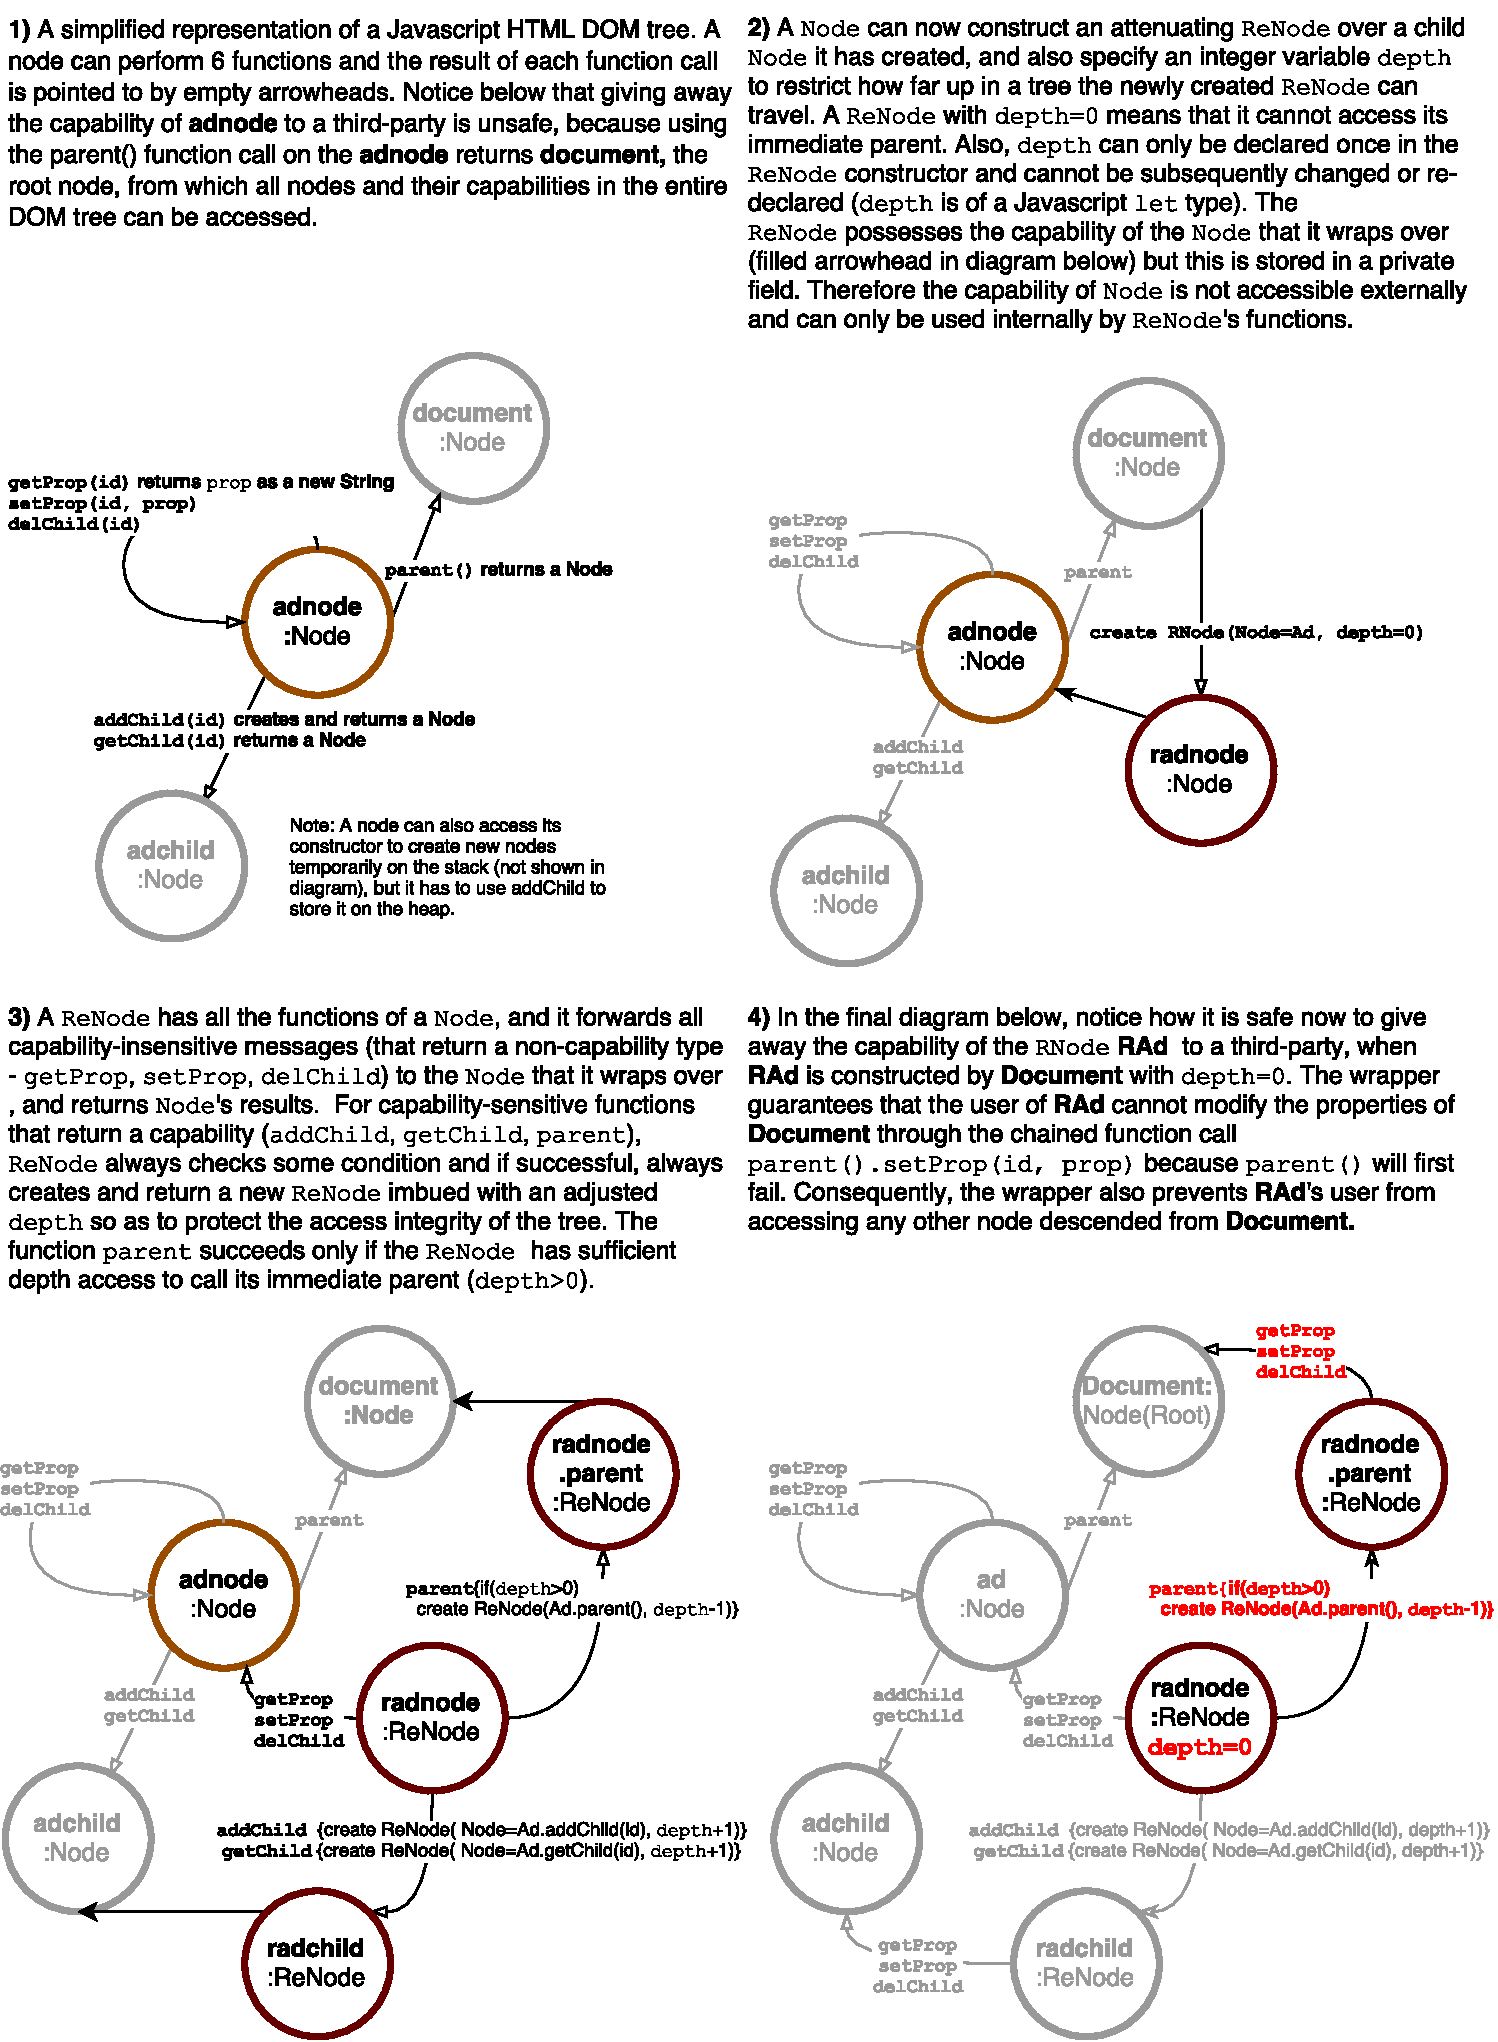
\includegraphics[width=1.05\textwidth]{figures/DOM.pdf}
 \captionof{figure}{JavaScript DOM Tree OCap Pattern}
  \label{DOM example}
\end{minipage}
\newpage\null\newpage
\section{Appendix}\label{appendix}
%----------------------------------------------------------------------------------------
%	REFERENCE LIST
%----------------------------------------------------------------------------------------
\small
\bibliographystyle{plain}
\bibliography{ref}

%----------------------------------------------------------------------------------------

\end{document}

